\documentclass[11pt,letterpaper]{article}
\usepackage[margin=17mm,top=21mm,bottom=18mm,headheight=14pt,headsep=8pt]{geometry}
\usepackage[T1]{fontenc}
\usepackage{helvet}
\renewcommand{\familydefault}{\sfdefault}
\usepackage{amsmath,amssymb,booktabs,array,tikz,fancyhdr,hyperref}
\usetikzlibrary{arrows.meta}
\hypersetup{colorlinks=true,urlcolor=blue!55!black,linkcolor=black}
\pagestyle{fancy}\fancyhf{}
\fancyhead[L]{\small Week 59 / Constant width / Facilitator guide}
\fancyfoot[L]{\footnotesize Bellingham Math Circle / Week 59 / W59-F-v1}
\fancyfoot[R]{\footnotesize\thepage}
\renewcommand{\headrulewidth}{0pt}\renewcommand{\footrulewidth}{0pt}
\setlength{\parindent}{0pt}\setlength{\parskip}{6pt}
\newcommand{\heading}[1]{\par\vspace{2pt}{\large\bfseries #1}\par}
\newcommand{\lead}[1]{\textbf{#1}}
\newcommand{\reuleaux}{\draw[line width=.6pt] (60,0) arc[start angle=0,end angle=60,radius=60] arc[start angle=120,end angle=180,radius=60] arc[start angle=240,end angle=300,radius=60] -- cycle;}
\begin{document}
\heading{Mathematical overview: the facts before the tasks}
\lead{Width is a whole-body support measurement.} For a nonempty compact convex filled shape $K$ and a unit vector $u$, its width is
\[
 W_K(u)=\max_{x\in K}x\cdot u-\min_{x\in K}x\cdot u.
\]
It is the perpendicular distance between two parallel lines that enclose the entire shape and both touch it. Translation does not change width. A line that cuts the shape is not a support. A slanted ruler reading, a chord through a mark, a radius and perimeter measure other quantities.

\lead{Exact constant-width theorem.} Start with an equilateral triangle of side $w>0$. Intersect the three closed disks of radius $w$ centered at its vertices. The boundary consists of three minor $60^\circ$ arcs, each joining two vertices with the third as center. This exact Reuleaux triangle has width $w$ in \emph{every} direction. The proof on page 2 checks both whole-body supports and covers all directions, including changes of contact at sector endpoints. An arbitrary rounded triangle need not have this property.

\begin{center}
\begin{tabular}{lrr}
\toprule Nominal full-size piece & Smallest width (mm) & Largest width (mm)\\\midrule
Disk, radius 30 & 60 & 60\\
Oval, ellipse $60\times40$ & 40 & 60\\
Square, side 60 & 60 & $60\sqrt2\approx84.853$\\
Equilateral triangle, side 60 & $30\sqrt3\approx51.962$ & 60\\
Reuleaux triangle, arc radius 60 & 60 & 60\\\bottomrule
\end{tabular}
\end{center}
\lead{Fixed gap and a marked point are different questions.} With translation allowed, a piece fits between ideal parallel lines at gap $g$ exactly when its width in that orientation is at most $g$; it can touch both exactly when its width equals $g$. At a fixed 60 mm gap, disk and Reuleaux triangle can turn with both contacts, oval and straight triangle can turn but lose simultaneous contact, and square cannot complete a turn.

The marked disk's center is always 30 mm from a support. The curved triangle's mark $O$ is the underlying equilateral centroid. Its perpendicular support distances range from $60-60/\sqrt3\approx25.359$ to $60/\sqrt3\approx34.641$ mm; opposite distances sum to 60. Constant width does not imply constant distances from a fixed mark, or constant height of an axle at that mark.

The curved triangle's three arcs each use one sixth of a radius-60 circle. Their total length is $60\pi$ mm, equal to the radius-30 disk's boundary. The direct arc argument suffices; no general perimeter theorem is needed.

\lead{Discovery and bands.} Pages 1--2 / Grades 2--5 invite children to choose orientations, find changing gaps and conjecture constancy. Pages 3--5 / ready Grades 3--5 add construction, all-direction explanation and the new marked-point measurement. Page 6 / ready Grades 4--5 uses sixths and scaling. Measurements are experiments; unequal legal gaps refute constancy, but equal sampled gaps do not prove it. There is no K--1 packet. All physical procedures, preparation estimates and classroom fit remain untested.

\newpage
\heading{Why the exact curved triangle has width $w$}
This is adult proof support for Problem 4, not a script to recite at the launch. Let $A=(0,0)$, $B=(w,0)$ and $C=(w/2,\sqrt3w/2)$, and let $K$ be the intersection of their three radius-$w$ disks. The intersection is compact and convex. On the circle centered at $A$, the points inside both other disks are exactly the minor arc $BC$; the other two circles give the other two arcs. Thus this is the whole boundary.

\lead{A whole sector, not a single drawing.} Let $u$ point anywhere between $AB$ and $AC$, endpoints included. Put $P=A+wu$. The angle between $u$ and either of the unit directions $AB,AC$ is at most $60^\circ$. Therefore
\[
 |P-B|^2=2w^2(1-\cos\phi)\le w^2,
\]
and the same holds for $C$. So $P\in K$ and is on arc $BC$. For every $x\in K$, $|x-A|\le w$, giving $x\cdot u\le w$, with equality at $P$. The perpendicular line through $P$ encloses and touches the entire shape.

\begin{center}
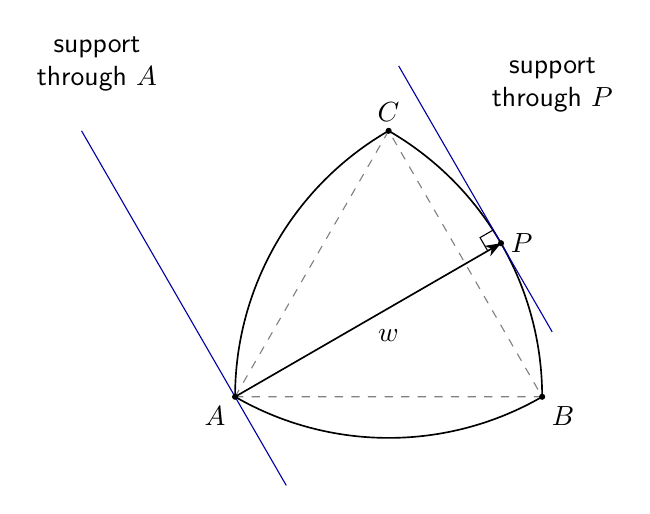
\begin{tikzpicture}[x=.65mm,y=.65mm,>=Stealth]
\reuleaux
\draw[gray,dashed] (0,0)--(60,0)--(30,{30*sqrt(3)})--cycle;
\draw[blue!65!black] (10,{-10*sqrt(3)})--(-30,{30*sqrt(3)});
\draw[blue!65!black] ({30*sqrt(3)+10},{30-10*sqrt(3)})--({30*sqrt(3)-20},{30+20*sqrt(3)});
\draw[->,line width=.6pt] (0,0)--({30*sqrt(3)},30) node[midway,below right] {$w$};
\draw ({30*sqrt(3)-3*.8660254},{30-3*.5})--({30*sqrt(3)-3*.8660254-3*.5},{30-3*.5+3*.8660254})--({30*sqrt(3)-3*.5},{30+3*.8660254});
\fill (0,0) circle[radius=.6] node[below left] {$A$};
\fill (60,0) circle[radius=.6] node[below right] {$B$};
\fill (30,{30*sqrt(3)}) circle[radius=.6] node[above] {$C$};
\fill ({30*sqrt(3)},30) circle[radius=.6] node[right] {$P$};
\node[align=center] at (-27,65) {support\\through $A$};
\node[align=center] at (62,61) {support\\through $P$};
\end{tikzpicture}
\end{center}
\lead{The vertex line really supports the whole body.} Expanding the disk inequalities $|x-B|^2\le w^2=|B|^2$ and $|x-C|^2\le w^2=|C|^2$ gives
\[
 x\cdot B\ge |x|^2/2\ge0,\qquad x\cdot C\ge |x|^2/2\ge0.
\]
Every $u$ in the closed sector is a nonnegative linear combination of $B,C$. Hence $x\cdot u\ge0$ for all $x\in K$, with equality at $A$. The parallel line through $A$ also encloses and touches the whole body. The gap between $x\cdot u=0$ and $x\cdot u=w$ is $w$.

\lead{Every direction is included.} The vertex-to-opposite-arc normal sectors are $[0^\circ,60^\circ]$, $[120^\circ,180^\circ]$ and $[240^\circ,300^\circ]$. Reversing $u$ leaves width unchanged and supplies $[180^\circ,240^\circ]$, $[300^\circ,360^\circ]$ and $[60^\circ,120^\circ]$. Together they cover the full turn. At a sector endpoint $P$ becomes a vertex; the same inequalities still apply. Both contacts may be vertices there. Three isolated examples, symmetry alone, or a radius touching only one line leave this proof incomplete.

\newpage
\heading{Preparation: a reusable kit, not weekly cutting}
Use the actual revised \texttt{students.pdf} (six pages, W59-S-v2) and \texttt{materials.pdf} (three pages, W59-M-v1). All material pages are US Letter, printed single-sided at 100\%. Compact student diagrams are sketches, not cutout patterns.

\begin{center}
\begin{tabular}{p{28mm}p{112mm}r}
\toprule Print & What each page supplies & Copies\\\midrule
Materials p.1 & Six full-size pieces: centered marked disk, oval, square, straight triangle, unmarked and centroid-marked Reuleaux triangles. & 5\\
Materials p.2 & One $200\times200$ mm mat with 10 mm grid. & 5\\
Materials p.3 & Two equilateral templates of each side length, 60 and 40 mm; optional construction. & 3\\\bottomrule
\end{tabular}
\end{center}
This is 10 basic material sheets and 3 optional sheets, \textbf{30 cut pieces}, five mats, and six templates of each size. Use flat 0.5--1 mm stiff card, or transfer the outlines to it. Cut along the middle of each thin outline; outside captions are not part of the piece. Keep the marked and unmarked curved pieces distinct. Adults do the initial cutting. Store one labeled reusable set per pair.

\lead{Each of five kits:} six pieces; two straight 300 mm rulers or rails with at least 100 mm unobstructed contacting edge; one 150 mm measuring ruler; two movable right-angle guides; one grid mat; pencil and blank paper. Totals: 10 rails, 5 measuring rulers, 10 right-angle guides, 5 mats. A folded square-corner card or set square is a proposed guide; it has not been rehearsed. Use the mat's perpendicular grid lines to check both rails against the same direction. Keep the piece flat, free to slide, with no center pin.

\lead{Optional construction:} six adjustable compasses, paper/templates, stiff-card backing if desired, and two pairs of adult-managed scissors, one at each older table. Six templates per size permit six makers; the seventh older child can check a partner's arc and swap. Children may share compasses in pairs. Compass-point management and cutting require the table adult; do not ask that adult to run several unfamiliar procedures simultaneously.

\lead{Student printing:} start with seven copies of pp.1--2 for the four third graders and three upper children. Print pp.3--6 only for the children choosing those continuations; three upper copies are a useful first reserve. K--1 use oral handling or an already familiar prior activity, not a new worksheet packet. Put one adult guide at each table. Keep all six student pages available for later visits.

\lead{Preparation estimate, untested:} allow roughly 60--90 minutes once for printing, transferring/cutting 30 shapes, assembling guides and packing five kits, plus 15--20 minutes for the physical rehearsal below. Later setup might take 10 minutes with stored kits. These are planning estimates, not measured timings; cutting speed and usable card may change them.

\lead{Rehearse before calling the kit ready.} Measure each 100 mm bar and both directions of the 200 mm mat; check 60/40 mm templates and actual cut dimensions. Test 300 mm rail clearance on the 200 mm mat and table, whole-body contact, parallelism, perpendicular readings and uninterrupted turns. For Problem 2 set and check the 60 mm gap at both rail ends, then secure the rails against movement while allowing piece translation; bring one roll of removable tape for this proposed setup. Check one-edge O-to-line measurement and a fixed compass opening. Printer margins, cutting, contact, rail gap, guides, compass procedures and timing are \textbf{unperformed}. A possible $\pm1$--$2$ mm apparent-width trial tolerance is only a proposal, not a verified guarantee. Do not silently widen the gap and report exact two-contact success.

\newpage
\heading{A concrete first hour at three fixed tables}
The group is eleven: K,K,1,1; 3,3,3,3; and 4,4,5. Three adults stay anchored: the parent volunteer at K--1, a mathematician at the third-grade table, and the organizer at the upper table. Allocate two kits to each younger table and one to the upper table. At the upper kit rotate chooser/turner, rail holder/measurer and contact referee. The referee checks rather than supplies the answer.

\lead{0--5 minutes:} the usual running-around transition. \lead{5--8:} let children handle pieces at their tables, compare outlines and try turning them, before adding measurement rules. \lead{8--12:} gather for a short shared demonstration. Use a scrap four-sided piece, not the target curved triangle. Place the two straight edges parallel, slide them until both touch and the whole piece is between them, then show a ruler held across the shortest gap. Use the student p.1 piece $\to$ parallel contacts $\to$ record visual: the nominal example's horizontal gap is 46 mm. Make one sketch and gap record. Children then choose the orientations.

Suggested launch words: ``Turn this piece. Slide these edges until both touch, with the whole piece between them. Keep the edges parallel. The shortest gap is its width in this position. Can you find a position with a smaller gap or a larger one?'' Keep the mathematical theorem for their later attempts.

\lead{12--32:} most older children use Problem 1. Let contrasting pieces receive real time; a partner can hold the guides while the chooser picks positions. Record only promising extrema and sketches, not a reading at every turn. \lead{32--50:} introduce Problem 2 to ready pairs; others continue the first investigation. Demonstrate the rule change on the scrap piece: set the gap to 60 mm and keep the rails fixed. A gap beside the piece is allowed. Ask separately about fitting and touching both. \lead{50--60:} share one changing-width witness and one conjectured constant-width piece; distinguish observations from reasons. These times are a proposed route, not a requirement to finish two pages.

\lead{Operational prerequisites.} For pp.1--2, children must choose/retain orientations, recognize enclosing parallel contact, use a perpendicular gap and compare whole-mm readings up to about 85. Adults may read prompts, record dictated answers and help alignment. Children must retain the choice of turns and comparisons. If the adult operates every turn and tells every result, switch to simpler concrete comparison or a familiar activity rather than pretending the independent investigation worked.

\lead{K--1 is an honest shallow entry.} With their anchored adult, children may choose a piece, turn it, bring two edges against it and compare ``wider here or there?'' only while they retain those choices. No numeric extrema, compass construction or universal proof is expected. If contact/parallelism requires repeated adult rescue, use the circle's previously successful pattern-block activity or another prepared familiar activity. Bring those materials separately. This is not claimed as a substantive K--1 constant-width packet; no new task is manufactured to fill a band.

\lead{Readiness-dependent continuations.} P3 requires fixed compass radius and equilateral side length; P4 needs tangent/radius perpendicularity and reasoning over intervening turns; P5 changes to one support and a marked point; P6 needs halves, sixths and length scaling by two. Adult reading is not the same as these reasoning prerequisites. The upper table may choose a continuation while the third graders finish P1--2; do not compress all six problems into one hour.

\lead{Record actual use.} Afterward note pages and pieces used, child-chosen positions, retained rules, adult rescues, conjectures and requested continuations. Separate observed behavior from explanations for it. Mark this new session unpiloted until actual use is recorded. Reusable materials can support several visits; finishing the packet is not the goal.

\newpage
\heading{Solutions and adult prompts: Problems 1--2}
\lead{Problem 1 / student p.1 / Grades 2--5.} Use the disk, oval, square, straight triangle and unmarked curved triangle; reserve the second marked curved copy for P5. The opening guidance applies to \emph{measuring width}: move the parallel edges into whole-body contact and measure perpendicularly. The worked parallelogram has vertices $(0,0),(38,0),(46,32),(8,32)$ in mm; the shown left/right supports are $x=0,46$, so the recorded gap is 46 mm. Its picture is at scale 0.55.

\lead{Expected ideal extrema} are the table on page 1. Nearest-mm physical records might be about 60/60, 40/60, 60/85, 52/60 and 60/60, respectively; those readings do not certify exact dimensions. For the oval its short and long axis directions witness the extrema. For the square side-normal contact gives 60, while a diagonal-normal direction gives $60\sqrt2$. For the straight equilateral triangle a side and opposite vertex give its altitude $30\sqrt3$; a side-parallel normal gives 60. For disk and exact curved triangle every orientation has width 60.

\lead{Why these are global extrema.} With normal angle $\theta$, ellipse width is $2\sqrt{900\cos^2\theta+400\sin^2\theta}$ and square width is $60(|\cos\theta|+|\sin\theta|)$. For the straight triangle, reversal and threefold symmetry give $60^\circ$ periodicity. In $0^\circ\le\theta\le30^\circ$ its width is $60\cos\theta$; in $30^\circ\le\theta\le60^\circ$ it is $60\cos(60^\circ-\theta)$. These include the switching endpoints and establish the listed bounds. Children can use side/vertex pictures rather than trigonometry.

\lead{Hints only when needed.} ``Which two places are touching?'' ``Does that edge cut through any part?'' ``Could your ruler cross the gap at a right angle?'' If extrema are missed, ask for a position very different from the current one, or offer the square on a corner and on a side as a comparison. A repeated equal reading is evidence for a conjecture, not proof. Small inconsistent readings first call for checking rails and cuts, not declaring a mathematical counterexample.

\lead{Problem 2 / student p.2 / Grades 2--5.} The rails now \emph{stay} 60 mm apart while the piece turns and slides. They enclose it, but need not both touch. Translation is allowed throughout; do not pin $O$ or any other point.
\begin{center}
\begin{tabular}{lcc}
\toprule Piece & Full turn inside? & Both contacts throughout?\\\midrule
Disk & Yes & Yes\\
Oval & Yes & No\\
Square & No & No\\
Straight triangle & Yes & No\\
Exact curved triangle & Yes & Yes\\\bottomrule
\end{tabular}
\end{center}
The oval's 40 mm position and triangle's altitude position refute continuous two-contact claims: sliding cannot increase a projection gap. The square's diagonal position obstructs a full turn. The ideal disk and curved triangle have width exactly 60 at every orientation. For the oval and triangle every width is at most 60; center their projection intervals in the strip at each angle to obtain a continuous translated full turn. This uses infinite ideal supporting lines; actual rail ends and hand clearance need a pretest.

\lead{Hint and explanation standard.} ``Can a piece fit with a gap beside it?'' ``Would sliding change the distance between its own supports?'' A deciding sketch can disprove a claim; one fitting sketch cannot prove an affirmative all-turn claim. Children may retain the affirmative outcomes as experimentally supported conjectures, then explain them using the width bounds or P4. If physical contact is ambiguous, record that limit separately from the ideal answer.

\newpage
\heading{Construction and explanation: Problems 3--4}
\lead{Problem 3 / student p.3 / ready Grades 3--5.} Use the full-size 60 and 40 mm equilateral templates on materials p.3. An equilateral triangle supplies three equal center-to-endpoint distances. Set the compass to one side $w$, and retain that opening for all three arcs:
\begin{center}
\begin{tabular}{lll}
\toprule Center & Endpoints joined & Short arc\\\midrule
$A$ & $B$ to $C$ & $60^\circ$\\
$B$ & $C$ to $A$ & $60^\circ$\\
$C$ & $A$ to $B$ & $60^\circ$\\\bottomrule
\end{tabular}
\end{center}
Each minor arc bulges outside its corresponding straight triangle side; retain the enclosed curved triangle, not the original straight triangle or the outside of all three disks. Adults can cut the resulting piece. Predicted exact widths are 60 mm and 40 mm. The smaller is a scale-$2/3$ copy of the larger. A child tests several orientations with adjustable touching supports, then compares the result with the prediction; cutting error is not a failure of the theorem.

\lead{Before compass use.} Student p.3 already shows a non-task example: $D=(0,0)$, $E=(25,0)$, $F=(0,25)$ mm; opening $DE$ at $D$ draws the short $90^\circ$ arc $EF$. Its display radius is 17.5 mm at scale 0.7. Demonstrate it on scrap if needed. It teaches fixed radius, not the three-arc construction's conclusion. Ask ``Where does the compass point go? Which two corners must the pencil reach?'' If the opening slips, let a partner check it against a side. A long $300^\circ$ arc or center on a side midpoint is a different construction. Optional return: let children diagnose such a deliberately altered scrap outline by finding a changing-width witness.

\lead{Problem 4 / student p.4 / ready Grades 3--5.} The student tangent convention precedes the task: a radius to a circle's single-contact tangent is perpendicular. The three printed curved triangles at $7^\circ,37^\circ,83^\circ$ illustrate positions, not complete angular coverage. The answer is the all-direction argument on page 2.

\lead{Concrete path to an explanation.} Let a child place legal supports on a construction-marked copy and choose the contact vertex. Lay a pencil segment from that vertex to the opposite arc contact. It is the generating radius. As that contact moves along the same arc, the segment stays $w$, and the two supports are perpendicular to it. Have the child check that the line through the vertex continues to enclose the whole piece, not just meet it. At the endpoint another vertex takes over; repeat for the other two centers and opposite normal directions. Offer the full sector drawing and inequalities only as needed for the adult's assurance.

\lead{Adult prompts.} ``Which corner made this arc?'' ``Could any part cross the line through that corner?'' ``What happens when the contact reaches an arc's end?'' ``Which turns have we still not explained?'' A good drawing or oral argument may supply the proof. Insist on both whole-body supports and intervening turns, without requiring coordinate notation from children. Accept the child's experimentally grounded conjecture if the universal explanation is beyond current readiness; keep P4 for a later visit.

\lead{Useful limits.} The exact assumptions are three equilateral vertices, equal radius equal to their side, and three minor arcs. Rounding a triangle by eye does not imply constant width. Radius perpendicular to one tangent proves only one support distance; the second support and sector coverage are essential. No axle, rolling platform, drill or square-hole procedure is involved.

\newpage
\heading{A marked point and one support: Problem 5}
\lead{Student p.5 / ready Grades 3--5.} Use the centered marked disk and centroid-marked curved triangle. The first-use visual is a different, off-center rectangle: $44\times28$ mm, mark $O=(12,9)$, right support $x=44$. The perpendicular ends at $(44,9)$ and measures $44-12=32$ mm. The total horizontal width would be 44 mm. All three panels use scale 0.6; the shown rectangle is $26.4\times16.8$ mm and measured segment 19.2 mm on the page. The 32 mm label records the nominal example, not a ruler reading from that compact sketch.

Before measuring the targets, use that visual to show the operational change: one edge encloses and touches the whole piece; put a right-angle guide at that edge and measure along its perpendicular through the mark. A slanted segment to a corner or the full two-edge gap answers a different question. Rotate and translate the whole marked piece; its mark remains attached.

\begin{center}
\begin{tabular}{lcc}
\toprule Marked piece & Smallest distance (mm) & Largest distance (mm)\\\midrule
Centered disk & 30 & 30\\
Centroid-marked curved triangle & $60-60/\sqrt3$ & $60/\sqrt3$\\
 & $\approx25.359$ & $\approx34.641$\\\bottomrule
\end{tabular}
\end{center}
\begin{center}
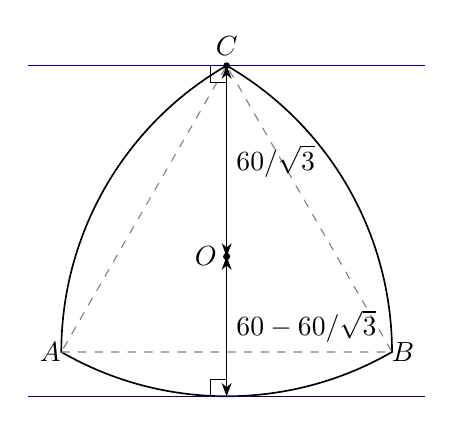
\begin{tikzpicture}[x=.7mm,y=.7mm,>=Stealth]
\reuleaux
\draw[gray,dashed] (0,0)--(60,0)--(30,{30*sqrt(3)})--cycle;
\draw[blue!65!black] (-6,{30*sqrt(3)})--(66,{30*sqrt(3)});
\draw[blue!65!black] (-6,{30*sqrt(3)-60})--(66,{30*sqrt(3)-60});
\fill (30,{10*sqrt(3)}) circle[radius=.65] node[left] {$O$};
\fill (30,{30*sqrt(3)}) circle[radius=.6] node[above] {$C$};
\draw[<->] (30,{10*sqrt(3)})--(30,{30*sqrt(3)}) node[midway,right] {$60/\sqrt3$};
\draw[<->] (30,{30*sqrt(3)-60})--(30,{10*sqrt(3)}) node[midway,right] {$60-60/\sqrt3$};
\draw (27,{30*sqrt(3)})--(27,{30*sqrt(3)-3})--(30,{30*sqrt(3)-3});
\draw (27,{30*sqrt(3)-60})--(27,{30*sqrt(3)-57})--(30,{30*sqrt(3)-57});
\node at (-2,0) {$A$};\node at (62,0) {$B$};
\end{tikzpicture}
\end{center}
The picture gives two attained extrema in one pair of supports. \lead{Why no other support is closer or farther:} put $R=w/\sqrt3=|O-A|$. In the $A$-sector of page 2, with $0^\circ\le\theta\le60^\circ$, the arc-side support distance from $O$ is
\[
 d_O(u)=w-R\cos(\theta-30^\circ).
\]
It ranges from $w-R$ at the sector midpoint to $w/2$ at its endpoints. The opposite distance is $w-d_O(u)=R\cos(\theta-30^\circ)$, ranging from $w/2$ to $R$. The other vertices and reversals cover every direction, so these are global bounds. The disk's support distance is its radius 30 in every direction. Answer: \textbf{yes}, constant width can coexist with changing marked-point distances.

\lead{Hints and limits.} ``Are you measuring from the mark or from the other edge?'' ``What changes when a corner, rather than an arc middle, touches?'' Let children search before offering the pictured witnesses. At nearest-mm precision expect roughly 25 and 35, with physical uncertainty. $O$ is not a common center of the three arcs. If an axle were placed there its support height would vary; this is a geometric consequence, not a tested rolling mechanism. An off-center disk mark would also vary, but the actual disk mark is centered. Total width fixes the sum of opposite distances, not each one separately.

\newpage
\heading{Boundary length: Problem 6, and return visits}
\lead{Student p.6 / ready Grades 4--5.} The generating circle has radius 60 mm, six equally spaced boundary dots and a highlighted $BC$ arc. Each Reuleaux boundary arc has that same radius and $60^\circ$ sweep, one sixth of this circle's circumference. Three such arcs total one half of the large circle's circumference. The comparison disk has radius 30 mm: scaling the generating circle by $1/2$ halves its entire boundary length. Therefore the two target boundaries are equal, both $60\pi\approx188.496$ mm. No decimal approximation to $\pi$ is needed for the exact comparison.

\lead{Hints.} ``How many copies of that short arc go around the large circle?'' ``How much of its boundary do the three arcs use?'' ``What happens to every length when the radius is halved?'' A string experiment can suggest equality but stretching, cutting and tracing cannot prove it. Keep the radius-60 construction circle distinct from the radius-30 disk. A wider-looking shape need not have a longer boundary.

\lead{Possible return sequence.} After a P1--2 first visit, choose P3 with predictions and two sizes, then P4 when contact centers and tangents have meaning. Another visit can focus on P5's new reference point and opposite-distance sum, followed by P6 for ready children. Let different tables return at different depths. Diagnose altered compass constructions or explore moving a disk's mark off center as adult-led continuations; do not add them as compulsory student substeps. Log actual pages used and prior conjectures so returning children resume a mathematical question rather than repeat a task unchanged.

\heading{Sources, adaptation and evidence limits}
\small
\lead{Mathematical/activity precedents consulted locally.} ThinkMaths, \href{https://think-maths.co.uk/resources/shapes-constant-width/}{\emph{Shapes of constant width}} (resource labels KS3, KS4, KS5); \href{https://think-maths.co.uk/wp-content/uploads/2023/03/Shapes-of-Constant-Width_0.pdf}{\emph{Shapes of Constant Width}}, PDF p.1, Activities 1--2: parallel-edge comparisons and contrasting rounded constructions. \href{https://think-maths.co.uk/wp-content/uploads/2023/03/Constructing-Shapes-of-Constant-Width.pdf}{\emph{Constructing Shapes of Constant Width}}, PDF p.1: equilateral vertices and radius equal to side. Francis E. Su et al., \href{https://math.hmc.edu/funfacts/reuleaux-wheel/}{\emph{Reuleaux Wheel}}, Harvey Mudd College Math Fun Facts, construction/constant-width paragraph and ``The Math Behind the Fact'': the established result and circumference-to-width claim. The complete support-sector proof here is independently derived; this packet uses only the direct three-arc perimeter argument. Source age labels and established theorems do not validate this elementary adaptation.

\lead{Actual teaching passages, then our inference.} Natasha Rozhkovskaya, \emph{Math Circles for Elementary School Students} (AMS, 2014), Lesson 6 ``At the lesson,'' ``Experiments with triangles and quadrilaterals,'' EPUB file \texttt{OEBPS/}\allowbreak\texttt{part0016.xhtml}, reports low child enthusiasm in the angle-cutting episode, while parents enjoyed it. Insufficient prior geometric experience is her proposed explanation, not an observed cause. Our inference is to give contrasting width examples time before expecting surprise or proof. Laura Givental, Maria Nemirovskaya and Ilya Zakharevich, \emph{Math Circle by the Bay} (AMS, 2018), Preface vii--ix (PDF pp.8--10): interaction (vii), deep themes (viii), clear understandable statements, manipulatives, independent solutions and difficulty verbalizing ideas (ix). Our inference is to preserve child-chosen turns and use adult alignment/reading assistance and optional explanation prompts. Neither passage pilots this session.

The organizer's prior \emph{Handouts 3.docx}, Problems 3.4--3.7, provides concrete tile/shape-comparison precedents; \emph{Pattern Block Exercises.pdf}, p.1 Problem 1, notes possible printed/material scale mismatch. These are not prior tests of this constant-width activity. Guide prose, figures and adaptation are newly authored around established mathematics. Downloaded references, books, workflow exemplars and older worksheets are not bundled. Root \texttt{REPUBLISHING.md} was read and preserved.

\lead{Digital versus physical evidence.} Nominal claims have the proofs above and a separate independent verifier. Revised student/material arcs are PDF cubic approximations: the sampled full-size disk widths are 60.000456--60.016920 mm; largest sampled Reuleaux nominal-width error is 0.001631 mm. These finite samples are not certified uniform bounds. All 100 mm bars, the 200 mm grid and both template sizes have been checked digitally. The guide's diagrams are equally scaled explanatory sketches, not new actual-size templates. Actual printer scale, stiff-card cuts/contact, rail clearance/parallelism/fixed gap, perpendicular measurement, compass operation, timing and classroom piloting remain \textbf{unperformed}. No physical smooth rolling, platform, axle or square-hole model has been tested.
\end{document}
